\documentclass{article}
\usepackage[utf8]{inputenc}
\usepackage[maxcitenames=1,style=numeric]{biblatex}
\usepackage{amsmath}
\usepackage{amssymb}
\usepackage{amsthm}
\usepackage{tcolorbox}
\usepackage{graphicx}
\usepackage{algorithm}
\usepackage{algorithmic}
\usepackage{subfig}
\usepackage{hyperref}
\usepackage{cleveref}
\usepackage{thmtools}
\usepackage{thm-restate}
\usepackage{enumerate}
\usepackage{xcolor}
\usepackage{textgreek}
\usepackage{caption}
%\usepackage{subcaption}

\topmargin -.5in
\textheight 9in
\oddsidemargin -.25in
\evensidemargin -.25in
\textwidth 7in

\title{Machine Learning based Translation Initiation Rate predictor}
\author{Zhang M., Holowko M. B., Hayman Zumpe H., Ong, C. S.}
\date{\today{}}

\bibliography{ref.bib}
\DeclareUnicodeCharacter{2212}{-}
\begin{document}

\maketitle

\section{Introduction}

One of the main tenets of synthetic biology is design, evaluation and standardisation of genetic parts \cite{Brophy2014,Canton2008,Stanton2014}.
This is usually done in terms of the Design-Build-Test-Learn (DBTL) cycle, where the given genetic part or organism are continually improved by going through a number of turns of the said cycle.
This normally involves designing the DNA sequence in Computer Aided Design (CAD) software and then physically testing it in a laboratory.
Additionally, computer modelling and prediction of part behaviour based on the designed DNA sequence or design of DNA sequence based on expected function can be used\cite{Yeoh2019,Nielsen2016}.
Most of these models are based on either the thermodynamic properties of the involved molecules (DNA, RNA, proteins, etc.) or empirically obtained values describing a relevant to a given design property, like Translation Initiation Rate (TRI) in case of Ribosome Binding Sites (RBS) \cite{Xia1998,Chen2013,Reeve2014}.
The biggest limitation for this approach currently is the Learn part of the cycle - there is very limited access to methods and software that can improve designs based on experimental results.\\
According to Reeve \emph{et al.} there are three main RBS calculators, all predicting the TRI based on the thermodynamic properties of the RBS and the ribosome \cite{Seo2013,Na2010,Salis2009}. 
Predictions from all of these models are relatively good ($R^2 >0.8$), but they come with a number of caveats: i) they rely on calculations of free energies that can be hard to estimate with high precision ii) in general, one of the best ways to improve the models' accuracy is by increasing the number of phenomenons taken into account, but this can lead to paradoxically decreased model accuracy due to accumulation of errors \cite{EspahBorujeni2016} and iii) by using deterministic coefficients to calculate energies one disregards often stochastic nature of processes in the cells which again increases perceived prediction error \cite{Goss1998}. \\
Synthetic biology is currently going through a phase of exponential increase in volume of data produced during experiments \cite{Freemont2019}. New experimental methods heavily relying on advances in automation and microfludics allow unprecedented precision and throughput in data generation.
These new data-sets can be combined with data reliant machine learning algorithms to generate new models and predictors for use in synthetic biology, vastly improving the DBTL cycle's performance \cite{Camacho2018}. In the past few years there was a significant uptake of Machine Learning based approaches in synthetic biology.
Jervis \emph{et al.} used support vector machine and neural network to optimise production of monoterpenoid in \emph{Esherichia coli} \cite{Jervis2019}. Similarly, Costello \emph{et al.} have used a number of machine learning approaches to analyse time-series multiomics data to predict metabolic pathway behaviour \cite{Costello2018}.
There were also successful attempts at using deep learning techniques for analysis of big data-sets \cite{Alipanahi2015,Angermueller2016}. However, the use of machine learning in synthetic biology is still in its infancy and will require additional research to show its full potential. \\
Here we present how machine learning algorithms can be used as part of the DBTL cycle to predict (Learn) and recommend (Design) variants of RBS with goal of optimization of protein level expression. RBS being one of the key genetic elements controlling protein expression and at he same time having a relatively short sequence is a perfect target for establishing workflows that can be later translated to more complicated systems.
We have used Gaussian Process-Upper Confidence Bound and multi-armed Bandits algorithms for prediction and recommendation respectively to analyse and optimise the initiation rates of the designed RBS. 
Our overall experimental goal was to maximise the Translation Initiation Rate (TIR) by identifying the set of RBS sequences with top TIR scores while minimising the number of DBTL cycle turns that we had to do.
We did this by designing a sequential experimental workflow, where we start with either randomised RBS sequences designed to explore the experimental space (designated round zero since only preexisting, literature data is used for its design) or with RBS sequences recommended by the algorithm (subsequent rounds). The designs were then physically constructed in batches of 90 to fit our automated process (see \textbf{Methods} section).
After constructing, the plasmids harbouring the new genetic devices are tested in microplate reader and flow cytometer. The results are then fed back to the algorithm for it to recommend the next round of designs.\\

\section{Method}
This will be about the DNA assembly.\\
\subsection{SynBio methods}
This will be very specifically talking about the plasmid.

\subsection{Algorithms}

\subsubsection{ Position probability matrix based sampling}


\subsubsection{Machine learning experimental design}

To automatically design the RBS sequences in batch using machine learning, we need to consider two parts: 
1) Design an regression algorithm which takes the RBS sequences as input and returns the predicted TIR scores and the confidence interval for the prediction. 
2) Design an online learning approach which recommends the RBS sequences based on the predicted TIR scores and confidence interval. 
Such online learning approach provides the $\textit{exploitation-exploration balance}$. 
We show the corresponding methods we use in the below. 

We consider our experimental design problem as the problem of sequentially optimising an unknown reward function $f: \mathcal{D} \rightarrow \mathbb{R}$, where $\mathcal{D}$ is the set containing all RBS sequence point, and $f(\mathbf{x})$ is the TIR score at $\mathbf{x}$. 
In each round $t$, we choose a set of $m$ points $\mathcal{S}_t \subset \mathcal{D}$ and observe the function values of each points in the selected set $\mathcal{S}_t$, i.e. $y_i = f(\mathbf{x}_i) + \epsilon_i$, for all $i \in \mathcal{S}$, where $\epsilon_i$ is the noise (we assume the noise is under Gaussian distribution with some unknown mean and variance). 
The noise influenced by the accuracy RBS calculator and other experimental interference (e.g. \textcolor{red}{To be added}). 
Our goal is to pick RBS sequence with the largest possible TIR score after the total number of rounds $N$. 

\begin{itemize}
    \item \textit{Gaussian process regression (GPR)}.
    A Gaussian process regression model \cite{Rasmussen2004} is a Bayesian approach to regression which provide uncertainty measurements on predictions. 
    We model $f$ as a sample from a \textit{Gaussian process} $GP(\mu(\mathbf{x}), k(\mathbf{x}, \mathbf{x'}))$, which is specified by the mean function $\mu(\mathbf{x})=\mathbb{E}[f(\mathbf{x})]$ and the kernel (or covariance) function $k\left(\mathbf{x}, \mathbf{x}^{\prime}\right)=\mathbb{E}[(f(\mathbf{x})-\left.\mu(\mathbf{x}))\left(f\left(\mathbf{x}^{\prime}\right)-\mu\left(\mathbf{x}^{\prime}\right)\right)\right]$.\\
    We choose to use \textit{spectrum kernel} \cite{leslie2001spectrum} to specify the kernel function of $GP$.  
    The spectrum kernel is widely used for classifying protein sequences \cite{leslie2001spectrum, ben2008support}, which takes two sequences as inputs and outputs a scalar value which represents the similarities between the two sequences. More precisely, $k_\ell^{\text{spec}}(\textbf{x}, \textbf{x}^\prime) =\left\langle\Phi_{\ell}^{\mathrm{spec}}(\mathbf{x}), \Phi_{\ell}^{\mathrm{spec}}\left(\mathbf{x}^{\prime}\right)\right\rangle$, where $\mathbf{x}, \mathbf{x}^\prime$ are two RBS sequences in $\mathcal{D}$ over an alphabet $\Sigma$. Denote the number of letters in the alphabet as $|\Sigma|$. $\Phi_{\ell}^{\mathrm{spec}}(\mathbf{x})$ maps the sequence $\textbf{x}$ into a $|\Sigma|^\ell$ dimensional feature space, where each dimension is the count of the number of one of the $|\Sigma|^\ell$ possible strings $s$ of length $\ell$.
    %Since the sequences in provided data have the pattern that the core area is different from each other, and other areas are similar. So the kernel for Gaussian Process we are using is the sum of kernels, for core areas we use spectrum kernel with string as input directly, and for other areas we use one-hot encoding and dot product kernel for simplicity.
    
    
    \item \textit{Upper confidence bound (UCB)}. Bandit algorithms \cite{lattimore2018bandit} provide various approaches to sequentially design an where an agent adaptively chooses one or more options among several actions based on certain policies. We consider a type of bandit algorithms, the upper confidence bound algorithm, which is based on the \textit{optimism in the face of uncertainty}. The UCB algorithm, as the name suggested, basically selects RBS sequences with the maximum upper confidence bound, i.e. $\operatorname{argmax}_{\mathbf{x}_i \in \mathcal{D}} \left( \mu_t(\mathbf{x}_i) + \beta_t \sigma_t(\mathbf{x}_i)\right)$,
    where $\beta_t$ is a hyperparmeter balancing the exploitation and exploration, 
    $\mu_t(\mathbf{x}_i), \sigma_t(\mathbf{x}_i)$ are the predicted mean and standard deviation at round $t$ for the sequence $\mathbf{x}_i$. 
\end{itemize}

Combine the two parts together, we apply \textit{Gaussian Process Upper Confidence Bound (GPUCB)} algorithm, which has been theoretically analysed by \textcite{srinivas2012information}. We show the flowchart of machine learning based experimental design in Figure \ref{fig: flowchart of machine learning based experimental design.}.


\begin{figure}[t]
    \centering
    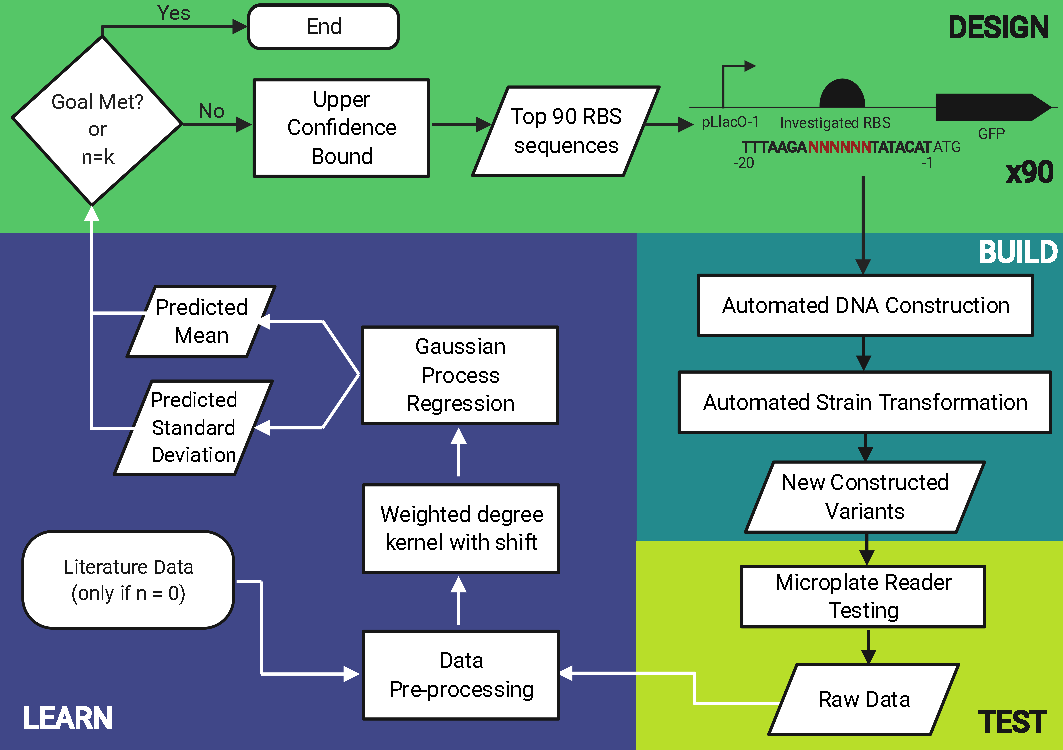
\includegraphics[scale=0.35]{plots/flowchart.pdf}
    \caption{Flowchart of machine learning based experimental design.}
    \label{fig: flowchart of machine learning based experimental design.}
\end{figure}







\section{Results}

Figure 1 shows the DBTL cycle with the machine learning process emphasised. Our machine learning workflow encompasses two phases of the cycle, namely the LEARN and DESIGN phase. In LEARN phase we use the Gaussian Process algorithm to predict the behaviour of different RBS sequences and in the DESIGN phase we use the multi-armed Bandit algorithm to recommend sequences to be Built and Tested next. Conventionally, the Design phase is considered the beginning of the cycle, however we will start description of our results from the learn phase, which we find a more natural starting point for a machine learning centred workflow.\\


\subsection{LEARN - prediction of RBS performance}
First problem to be tackled was how to embed the sequence to give our RBS sequences numerical form. As we will be using a Gaussian Process for regression we have investigated use of different types of kernels (also called covariances) for embedding \cite{Ben-Hur2008}. The additional, and positive, effect of using kernels is that our data will be moved to a higher-dimensional space, which makes the regression process easier. We compared performance of Dot Product, RBF and a number of string kernels: spectrum, mixed spectrum, weighted degree and weighted degree with shifting \textcolor{red}{Figure Xa}. Since we found that the spectrum kernel performed the best, we have used it in subsequent studies. More specifically, we used a summary of three kernels: spectrum kernel to process the core 6bp and dot product kernel to process the 7bp flanking sequences both upstream and downstream of the core sequence. This approach allowed for good balance between computational complexity and performance.\\
The predictions were made using the Gaussian Process regression (GPR) algorithm. In essence, Gaussian Process is a stochastic (Bayesian) predictor of the shape of a function, which is built based on  perceived similarities between data points (kernels), where not only a mean value, but also probability distribution of the mean is calculated. Such an approach makes GPR well suited to predict biological phenomena which are also highly stochastic. \\
For the zeroth round, since we don't have access to any prior data fitting our design we approximated the predictions using the data from \textcite{jervis2018machine} and the Gaussian Process regression method (see \textbf{Methods} section) \cite{srinivas2012information}. This set contains 113 non-repeated records for 56 unique RBS sequences with the respective TIR. The label values are between 0 - 100,000 and skewed, which is shown in Figure xx. First, we have normalised the label to 0 - 1 using the min-max normalisation. The predictions are shown in \textcolor{red}{Figure Xb}\\
The predictions for next rounds were predicted similarly, but with use of data obtained in previous rounds, visualisation of prediction for the last round of designs is shown in \textcolor{red}{Figure Xc} \\

\subsection{DESIGN of the genetic device}
There is a number of factors that impact the protein expression rate, many of them concerned with how the ribosome recognises and binds to the RBS sequence \cite{Chen1994,Vellanoweth1992}. In \emph{E. coli} the RBS is usually located in the 20 bases upstream of the start codon. The RBS usually has a distinguishable, consensus, core sequence called the Shine-Dalgarno sequence, which in \emph{E. coli} is AGGAGG. Here, we put that 20 bp long sequence into focus with main emphasis being put on the 6bp core region (Figure \ref{fig:Anatomy}).\\

\begin{figure}[h]
    \centering
    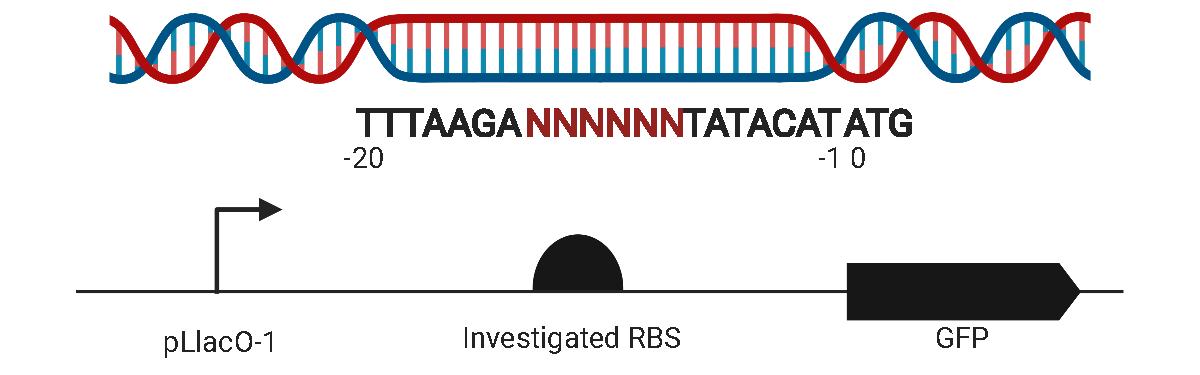
\includegraphics[scale=0.6]{plots/RBS_anatomy.pdf}
    \caption{\textbf{Diagram of the investigated sequence.} The sequence of the investigated RBS is shown with the randomised core sequence in red. The start codon of the GFP coding sequence is also shown with numbers showing relative nucleotide positions.}
    \label{fig:Anatomy}
\end{figure}

In our genetic design, the investigated RBS controls expression of the Green Fluorescent Protein (GFP) in its mut3b variant. By controlling expression of a fluorescent protein with the RBS we can quickly assess the perceived TIR by measuring fluorescence of cells harbouring plasmid with the device. Finally, the mRNA is transcribed from an IPTG-inducible promoter pLlacO-1. By making the whole device inducible we can synchronise the start of the expression of the GFP in all the cultures by inducing them at the same optical density (OD\textsubscript{600}) with addition of IPTG.\\
The investigated RBS sequence is 20 bps long with the sequence TTTAAGAAGGAGATATACAT, which is a known high TIR RBS that comes with the pBb series plasmids \cite{Lee2011}. In our design we focus on randomising of the core -8 to -13 (relative to the GFP) nucleotides of the RBS and fix others to be the same as the consensus sequence, i.e. TTTAAGA + NNNNNN + TATACAT. Since for each of the 6 position there are 4 possibilities: A, C, G, T the total variant space is $4^6$ = 4096.\\
Since there was no prior data that we could have used to guide our design for the zeroth round of experiments, we have designed 180 (two times 90) RBS sequences based on the consensus sequence that we expected to give good cover of the experimental space: 

\begin{enumerate}
    \item 60 RBS sequences which are subsequent single nucleotide changes of all 20 nucleotides of the original, consensus sequence. This batch is designed to show us influence of such single nucleotide changes on the overall performance of the RBS and the potential impact of changes made beyond the core part.
    \item 30 RBS sequences that were fully and uniformly randomised (equal probability of choosing either nucleotide for each position) 
    \item 30 RBS sequences randomised based on the position probability matrix (PPM) \textcolor{red}{we need a citation and better explanation for this}  
    \item 60 RBS sequences recommended by our multi armed bandit recommendation algorithm based on the initial literature, as described below.
\end{enumerate}{}

\begin{figure}[t]
    \centering
    \includegraphics[scale=0.7]{plots/TIR_histogram.pdf}
    \caption{TIR Histogram.}
    \label{fig: TIR Histogram.}
\end{figure}

\begin{enumerate}
    \item RMSE of predictions.
    
    \item Similarity of recommendations. 
    \begin{figure}[t]
    \centering
    \includegraphics[scale=0.7]{plots/similarity_first_round_recommendation.pdf}
    \caption{TIR Histogram.}
    \label{fig: TIR Histogram.}
\end{figure}
\end{enumerate}{}

The bandit algorithm aims at maximising the reward (output) from testing a limited number of instances from a big pool which cannot be wholly tested due to limited resources (time, computational power, capital). As such, it is very useful in solving problems like the one presented here - a big pool of potential designs, but only limited time and money that can be used for finding the optimal one.\\
In short, the multi-armed bandit algorithm is a stochastic method of probing of the experimental space. In our case we use the Upper Confidence Bound version of the algorithm, which focuses its recommendations on sequences that should give highest TIR based on the probabilities computer by the prediction algorithm (GPR). Another feature of the bandits algorithms is that it balances two approaches: exploration and exploitation. Exploration makes the algorithm to recommend designs that will improve the predictions better, whereas exploitation will recommend designs that focus on delivering the most efficient design the fastest. The two approaches can be controlled with the \textbeta\enspace parameter. We have decided that in the first iterations of the cycle it would be beneficial to skew the algorithm towards the exploration with exploitation taking increasing role in later iterations. One thing of note is that the bandit algorithm is stochastic, that is it exploits the probabilities of given event occurring (in this case RBS having a specific TIR). As such, it pairs naturally with our prediction algorithm, the Gaussian Process, which provides probability based function regression.\\
\\
For rounds beyond the initial, zeroth one, the designs were recommended only by the bandit algorithm based on the data obtained in the previous one, without adding any random designs. In total, three more rounds beyond the initial one have been performed, each with designs recommended by the algorithm. 

\subsection{BUILD and TEST}

For the machine learning to work effectively the analysed data-set needs to show two qualities: high relative volume and high quality of data.
These two elements don't have a specific definitions, but in general the data-set have to be going into at least hundreds possible data points and one have to cover 5-10\% of that space.
And since quality of the obtained data has a direct and strong correlation with quality of the predictions and in effect - recommendations, one need to ensure that the obtained results represent the real value as close as possible.\\
To help us obtain reliable and reproducible results we have employed automation-heavy workflow for our experiments.
This way we hope to eliminate a big part of sample-to-sample variation as well as human-introduced variation.
Additionally, performing all the procedures directly in 96-well microplate format enabled us to significantly cut down time to prepare our variants.\\
In short, the genetic variations of the RBS were introduced to the plasmids with combination of PCR and isothermal assembly.
The plasmids were then transformed and the resulting transformants were tested both using microplate reader and flow cytometry.\\
Figure X shows the results of the zeroth and all the subsequent rounds.\\

\subsection{EXIT}
There are two potential points where the exit from the cycle should be considered: i) the optimum solution has been found or ii) depletion of available resources (time and/or money). In our case we have performed a total of four rounds, with performance of the RBSes increasing as seen in \textcolor{red}{Figure X}.\\

\section{Summary}

\section{Contributions}
Zhang M. and Ong C. S. designed and implemented the machine learning algorithms and workflow. Holowko M. B. and Hayman Zumpe H. have designed and performed the laboratory experiments. All authors contributed to and reviewed the manuscript.


\newpage

\printbibliography

\clearpage

\appendix
\section*{Appendix}

\section{Choices of Kernels}

\begin{itemize}
    \item Spectrum Kernel.
    \item Mixed Spectrum Kernel.
    \item Weighted Degree Kernel. 
     $\overline{\mathbf{x}}, \overline{\mathbf{x}}^{\prime}$ are two sequences over an alphabet $\Sigma,$ e.g., RBS sequences. By $|\Sigma|,$ we denote the number of letters in the alphabet. $\phi_{\ell}^{\text {Spec}}$ is a mapping of the sequence $\overline{\mathbf{x}}$ into a $|\Sigma|^{\ell}$ dimensional feature space. Each dimension corresponds to one of the $|\Sigma|^{\ell}$ possible strings $s$ of length $\ell$ and is the count of the
    number of occurrences of $s$ in $\overline{\mathbf{x}}$. 
    For sequences with fixed length $L$ and weighted degree kernel consider substrings starting at each position $l = 1, ..., L$, with $\beta_d = \frac{2(\ell - d + 1)}{\ell(\ell+1)}$, \\
    \textit{Vector input}: 
    \begin{align}
        k_\ell^{WD}(\overline{\mathbf{x}}, \overline{\mathbf{x}}^\prime) 
        &= \sum_{d=1}^{\ell} \sum_{l=1}^{L-d+1} \beta_d k_d^{Spec}(\overline{\mathbf{x}}_{[l:l+d]}, \overline{\mathbf{x}}_{[l:l+d]}^\prime)\\
        &= \sum_{d=1}^{\ell} \sum_{l=1}^{L-d+1} \beta_d \phi_d^{Spec}(\overline{\mathbf{x}}_{[l:l+d]})^T \phi_d^{Spec}(\overline{\mathbf{x}}_{[l:l+d]}^\prime)\\
        &= \sum_{d=1}^{\ell} \sum_{l=1}^{L-d+1} \beta_d \mathbb{I}(\overline{\mathbf{x}}_{[l:l+d]} = \overline{\mathbf{x}}_{[l:l+d]}^\prime),
    \end{align}
    where $\mathbb{I}(\text{true}) = 1$ and 0 otherwise. 
    \textit{Matrix input}: $\mathbf{X}, \mathbf{X}^\prime$ are two metrics which includes $n$ sequences, and $\Phi_d^{Spec}(\mathbf{X}) \in \mathbb{R}^{n \times |\Sigma|^{\ell}}$.
    \begin{align}
        K_\ell^{WD}(\mathbf{X}, \mathbf{X}^\prime)
        = \sum_{d=1}^{\ell} \sum_{l=1}^{L-d+1} \beta_d \Phi_d^{Spec}(\mathbf{X}_{[:, l:l+d]}) \Phi_d^{Spec}(\mathbf{X}_{[:, l:l+d]}^\prime)^T
    \end{align}
    
    \item Weighted Degree Kernel With Shift.
    \begin{align}
        k_\ell^{WDS}(\overline{\mathbf{x}}, \overline{\mathbf{x}}^\prime) 
        &= \sum_{d=1}^{\ell} \beta_d \sum_{l=1}^{L-d+1} \gamma_l \sum_{s = 0, s + l \leq L}^{S(l)} \delta_s
        \left(k_d^{Spec}(\overline{\mathbf{x}}_{[l+s:l+s+d]}, \overline{\mathbf{x}}_{[l:l+d]}^\prime) + (k_d^{Spec}(\overline{\mathbf{x}}_{[l:l+d]}, \overline{\mathbf{x}}_{[l+s:l+s+d]}^\prime)\right)\\
        &= \sum_{d=1}^{\ell} \beta_d \sum_{l=1}^{L-d+1} \gamma_l \sum_{s = 0, s + l \leq L}^{S(l)} \delta_s
        \left(\mathbb{I}(\overline{\mathbf{x}}_{[l+s:l+s+d]} = \overline{\mathbf{x}}_{[l:l+d]}^\prime) + (\mathbb{I}(\overline{\mathbf{x}}_{[l:l+d]}= \overline{\mathbf{x}}_{[l+s:l+s+d]}^\prime)\right),
    \end{align}
    where $\beta_d = \frac{2(\ell - d + 1)}{\ell(\ell+1)}, \delta_s = \frac{1}{2(s+1)}$, $\gamma_l$ is a weighting over the position in the
    sequence, which we set to 1. $S(l)$ determines the shift
    range at position $l$.
\end{itemize}

\textbf{From kernel to distance}:
$$d(\overline{\mathbf{x}}, \overline{\mathbf{x}}^\prime) = \sqrt{k(\overline{\mathbf{x}}, \overline{\mathbf{x}}) + k(\overline{\mathbf{x}}^\prime, \overline{\mathbf{x}}^\prime) - 2 k(\overline{\mathbf{x}}, \overline{\mathbf{x}}^\prime)} $$

\section{Design Choices}

\begin{itemize}
    \item Embedding.
    \item Kernel.
    \item Regression model.
    \item Bandit model.
\end{itemize}

\section{Intuition behind UCB and visualisation}

\begin{itemize}
    \item Exploitation and exploration explanation.
    \item Visualise coverage by clustering plot.
    \item Table for in-clustering mean and variance.
\end{itemize}

\section{Result analysis}

\begin{itemize}
    \item violinplot.
    \item regression performance plot, table.
    \item kernel matrix plot.
\end{itemize}

\section{Figures}




\end{document}
